\chapter{Razvojni sustav ESP32-C3-DevKitM-1}

Razvojni sustav temelji se na modulu ESP32-C3-MINI-1. Modul je jedan u nizu ESP32-­C3 serije SoC (engl. \textit{System on Chip}) platformi tvrtke \textit{Espressif}, te sadrži jednojezgreni 32-bitni procesor s RISC-V arhitekturom koji radi na frekvenciji do 160 MHz. Modul sadrži 400 KB memorije tipa SRAM (engl. \textit{Static random-access memory}), od kojih je 16 KB rezervirano za priručnu memoriju (engl. \textit{cache}), 384 MB memorije tipa ROM (engl. \textit{Read-only memory}) te 4 MB memorije tipa \textit{Flash}. Od periferije sadrži 22 programabilna GPIO pina (engl. \textit{General Purpose Input Output}), te digitalna sučelja SPI, UART, I2C i I2S. Također sadrži upravljače za sučelja USB i JTAG koji se mogu koristiti za efikasnije otklanjanje pogrešaka u kodu (engl. \textit{debugging}). Konfiguracija sustava prikazana je na slici \ref{fig:esp32}. \cite{esp32manual}

\begin{figure}[ht]
	\centering
	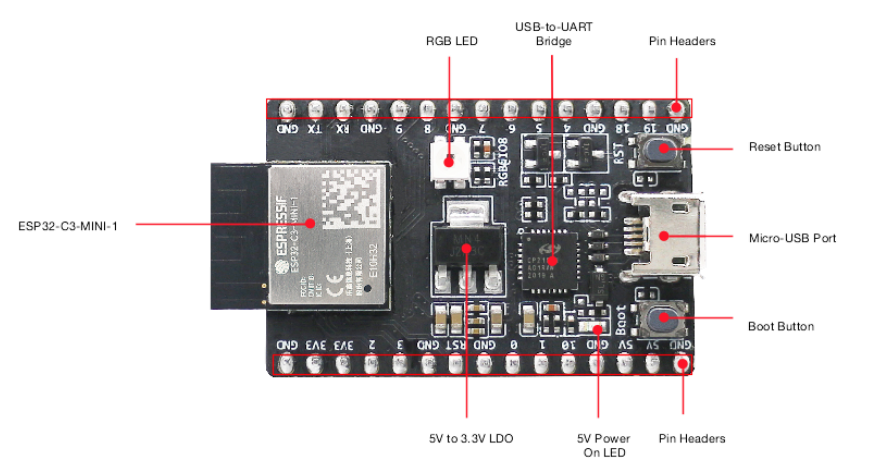
\includegraphics[scale=0.6]{imgs/esp32}
	\caption{Konfiguracija razvojnog sustava ESP32-C3-DevKitM-1 \cite{espressif}}
	\label{fig:esp32}
\end{figure}

Budući da modul ima funkciju RF (engl. \textit{radio frequency}) primopredajnika, podržava bežično lokalno umrežavanje odnosno Wi-Fi, koji omogućava propusnost do 20 Mbps protokolom TCP te maksimalnu propusnost od 30 Mbps koristeći protokol UDP. Isto tako, podržava protokol Bluetooth s podrškom za velike udaljenosti. 

Modul ESP32-C3-MINI-1 bežični je uređaj niske potrošnje energije (engl. \textit{ultra-low-power}) primarno namijenjen razvoju aplikacija koje koriste Wi-Fi ili \textit{Bluetooth Low Energy} (BLE) protokol. Na slici \ref{fig:esp32block} nalazi se blok shema modula sa svim dostupnim značajkama. 

\begin{figure}[ht]
	\centering
	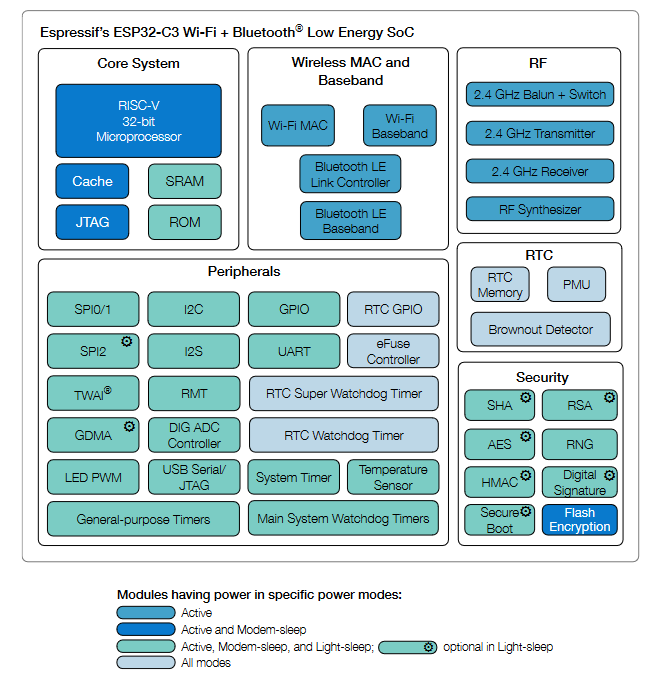
\includegraphics[scale=0.6]{imgs/esp32block}
	\caption{Blok dijagram modula ESP32-C3 \cite{esp32manual}}
	\label{fig:esp32block}
\end{figure}

\section{Wi-Fi}

IEEE 802.11, skupina standarda za bežične lokalne mreže (engl. \textit{WLANs}) \cite{ieee}, nudi nekoliko različitih načina bežične modulacije signala. Pojedini standardi označeni su slovima abecede. Za korisničke mreže postoje dva frekvencijska pojasa: 2,4 GHz i 5 GHz. 

Prednosti pojasa od 2,4 GHz su veći doseg, bolje prolaženje kroz fizičke prepreke te bolja podrška jer više bežičnih uređaja koristi pojas od 2,4 GHz nego od 5 GHz. S druge strane, ovaj pojas ima manju propusnost i nudi manje kanala koji se ne preklapaju. Isto tako, može doći do zagušenja mreže jer kućni i Bluetooth uređaji koriste ovaj isti mrežni pojas.

Pojas od 5 GHz nudi brži protok, manje zagušenih kanala te ima više kanala koji se međusobno ne preklapaju. Ipak, ima kraći raspon u usporedbi s mrežama od 2,4 GHz jer teže prolazi kroz prepreke. \cite{microsoft_ieee} 

U nastavku su opisani ključni standardi Wi-Fi tehnologije \cite{how_wifi_works}:
\begin{itemize}
	\item 802.11b - najsporiji i najjeftiniji standard, emitira u frekvencijskom pojasu od 2,4 GHz. Može prenijeti do 11 Mbps te koristi komplementarno šifriranje (engl. \textit{complementary code keying - CCK}) radi poboljšanja brzine prijenosa.
	\item 802.11a - transmitira u pojasu od 5 GHz i može prenijeti do 54 Mbps. Koristi ortogonalno frekvencijsko multipleksiranje (engl. \textit{orthogonal frequency-division multiplexing - OFDM}), što je efikasnija tehnika u odnosu na CCK koja dijeli radio signal u nekoliko podsignala prije slanja primatelju. Ova metoda značajno umanjuje interferenciju. 
	\item 802.11g - poput standarda 802.11b, koristi frekvencijski pojas od 2,4 GHz. Međutim, može prenijeti do 54 Mbps jer koristi tehniku OFDM.
	\item 802.11n - kompatibilan je standard sa prethodno opisanim standardima. Nudi znatno poboljšanje u rasponu i brzini u odnosu na svoje prethodnike. Ovaj standard može prenijeti do četiri toka podataka, svaki maksimalno 150 Mbps, no većina usmjerivača (engl. \textit{router}) dopušta dva ili tri toka.
	\item 802.11ac - radi isključivo u pojasu od 5 GHz, te je kompatibilan s prethodnim standardima. Manje je sklon interferenciji i brži je od prethodnih standarda s maksimalnim prijenosom od 450 Mbps jednim tokom. 
	\item 802.11ax - najnoviji standard koji proširuje nekoliko ključnih mogućnosti svojih prethodnika. Usmjerivači koji podržavaju ovaj standard dopuštaju tok podataka do 9.2 Gbps, što je značajan porast u usporedbi s prethodnicima. Isto tako, moguće je postaviti više antena na jedan usmjerivač, čime je omogućen prihvat više veza odjednom bez usporavanja i interferencije.
\end{itemize}

Podsustav modula za Wi-Fi u skladu je sa standardom IEEE 802.111 te koristi nelicencirani pojas frekvencija od 2,4 GHz. U tom pojasu podržava propusnost od 20 i 40 MHz. Modul također podržava tehniku raznolikosti antena (engl. \textit{antenna diversity}) za poboljšanje prijema i pouzdanosti signala korištenjem RF komutatora (engl. \textit{switch}). Tim komutatorom upravljaju GPIO priključci i koristi se za odabir najbolje antene u kontekstu pouzdanosti i kvalitete signala. \cite{esp_mini}

ESP32-C3 u potpunosti implementira Wi-Fi protokol na temelju standarda 802.11 b/g/n. Podržava osnovni skup (engl. \textit{Basic Service Set - BSS}) operacija za značajke pristupne točke (engl. \textit{SoftAP}). Upravljanje napajanjem odvija se automatski s minimalnom intervencijom domaćina kako bi se smanjila aktivnost uređaja.

Tvrtka \textit{Espressif} također nudi biblioteke za povezivanje putem protokola TCP i IP te korištenje Wi-Fi \textit{mesh} tehnologije. Pruža i podršku za protokole TLS 1.0, 1.1 i 1.2. Na slici \ref{fig:wifi_rf_table} prikazani su Wi-Fi RF standardi koje koristi modul. 

\begin{figure}[ht]
	\centering
	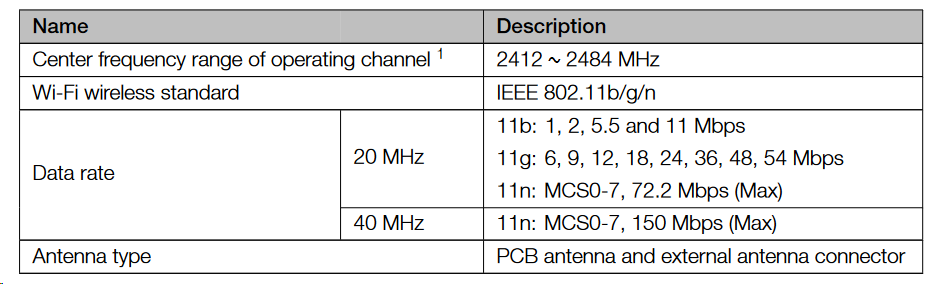
\includegraphics[scale=0.5]{imgs/wifi_rf_table}
	\caption{Wi-Fi RF standardi \cite{esp_mini}}
	\label{fig:wifi_rf_table}
\end{figure}

ESP32 nudi nekoliko načina rada pri korištenju Wi-Fi tehnologije \cite{esp_wifi_connect_overview}:
\begin{enumerate}
	\item način rada stanice - ESP32 spaja se na točku pristupa (engl. \textit{station mode}),
	\item način rada pristupne točke - druge se stanice spajaju na ESP32 (engl. \textit{SoftAP mode}),
	\item miješani - ESP32 radi kao stanica i pristupna točka spojena na drugu pristupnu točku. 
\end{enumerate}

U nastavku su opisani scenariji Wi-Fi povezivanja modula ESP32-C3 u načinu rada stanice i pristupne točke.

Na slici \ref{fig:station_scenario} prikazan je sekvencijski dijagram zadataka koje ESP32 obavlja u cijelom ciklusu spajanja i komunikacije s pristupnom točkom. Iz slike je vidljivo da se ciklus sastoji od osam faza. Prva faza služi za inicijalizaciju upravljačkih programa i pokretanje zadataka odnosno dretvi koje će obavljati zadatke vezane uz svoju dužnost. Glavni zadatak pokreće četiri različite dretve izvršavanja: aplikacijski zadatak, zadatak za događaje, zadatak za IP protokol, te zadatak za Wi-Fi. U drugoj fazi konfigurira se upravljački program za Wi-Fi. U sljedećoj se fazi pokreće upravljački program, nakon koje slijedi faza pretraživanja mreže i povezivanja na usmjerivač ili pristupnu točku. Nakon inicijalizacije DHCP klijenta, započinje faza dohvata IP adrese. Šesta faza odvija se nakon prekida Wi-Fi veze, čime se također uklanjaju i sve UDP i TCP konekcije. U aplikaciji se može omogućiti radno čekanje na ponovno uspostavljanje veze. Sedma faza pokreće se pri detekciji promjene IP adrese. Posljednja faza služi za programsko odspajanje s mreže i zaustavljanje upravljačkog programa za Wi-Fi.

Slika \ref{fig:ap_scenario} modelira slučaj u kojem ESP32 ima ulogu pristupne točke. Scenarij je vrlo sličan ranije opisanom slijedu događaja, no razlikuje se u dvije faze i događajima koji su pohranjeni u sustavu. Ovaj način rada nema fazu detekcije promjene IP adrese, jer je u ovom načinu ESP32 upravo taj uređaj čija se IP adresa može promijeniti. Isto tako, ne postoji faza dohvata IP adrese. 

\begin{figure}[ht]
	\begin{minipage}[t]{0.4\textwidth}
		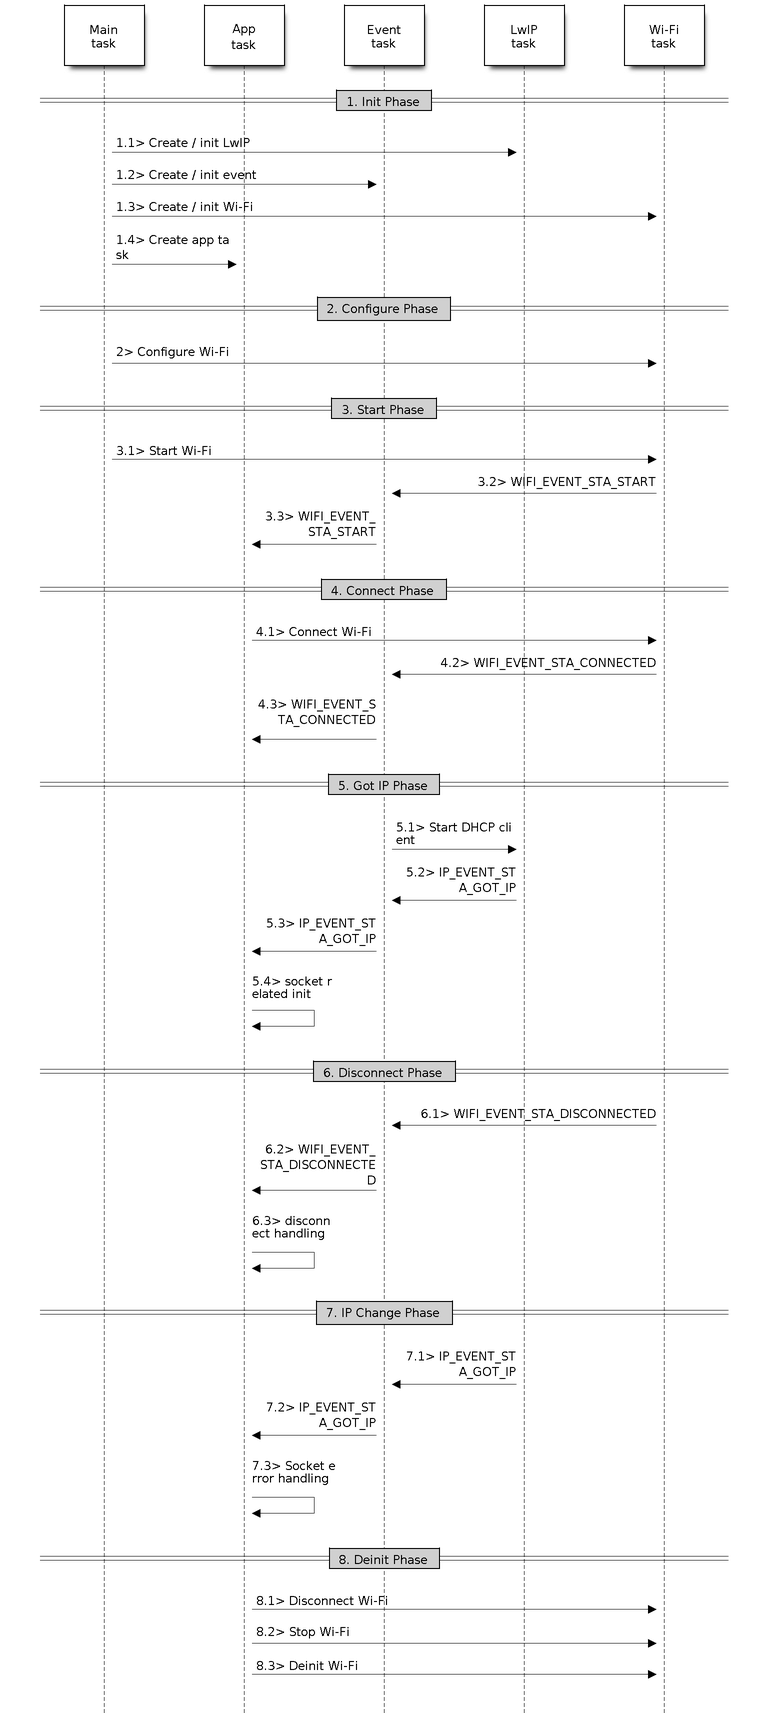
\includegraphics[width=\linewidth]{imgs/station_scenario}
		\caption{Primjer scenarija Wi-Fi povezivanja u načinu rada stanice \cite{espressif}}
		\label{fig:station_scenario}
	\end{minipage}
	\hspace*{\fill}
	\begin{minipage}[t]{0.4\textwidth}
		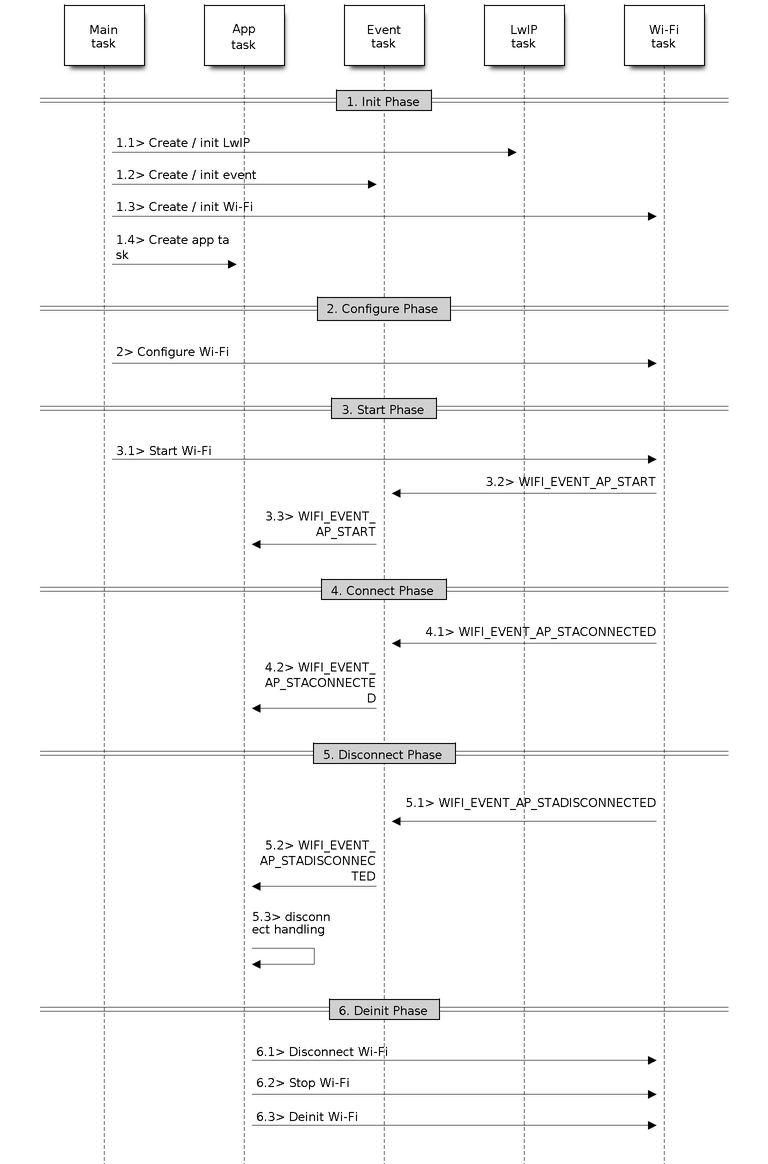
\includegraphics[width=\linewidth]{imgs/ap_scenario}
		\caption{Primjer scenarija Wi-Fi povezivanja u načinu rada pristupne točke \cite{espressif}}
		\label{fig:ap_scenario}
	\end{minipage}
\end{figure}

U modulu ESP32 stavljen je veliki naglasak na mehanizme uštede energije, što se također preslikava na korištenje Wi-Fi veze. Modul pruža načine uštede energije i pri radu kao stanica i pristupna točka, no neke značajke nisu podržane u pristupnoj točki. Modul pri neaktivnosti može otići u stanje mirovanja (engl. \textit{sleep mode}). Postoje dva načina uštede energije u načinu rada stanice: minimalna i maksimalna ušteda. Pri minimalnoj uštedi stanica se budi iz stanja mirovanja nakon svakog DTIM intervala (engl. \textit{Delivery Traffic Indication Message}). Ovim se načinom ne gube globalno emitirane poruke (engl. \textit{broadcast}) jer se one prenose nakon DTIM intervala. Međutim, ova metoda ne štedi puno energije ako je pristupna točka na koju je spojen modul postavila malen interval. Pri maksimalnoj uštedi moguće je znatno produžiti vrijeme mirovanja u odnosu na DTIM interval, no ovime se riskira gubitak globalno emitiranih poruka. 

\section{Aplikacijska programska sučelja}

Aplikacijska programska sučelja (engl. \textit{Application Programming Interface - API}) služe za olakšano korištenje usluga, protokola i periferija koje nudi hardver. Dostupno je mnogo API-ja za ESP32-C3 \cite{espressif}, no ovdje je napravljen osnovni pregled programskih sučelja koja koriste Wi-Fi. Ova sučelja nude proširenja na bazni upravljački program za povezivanje putem Wi-Fi mreže.

\textit{Wi-Fi Easy Connect}, također poznat kao prokol za provizioniranje uređaja (engl. \textit{Device Provisioning Protocol - DPP}) ili \textit{Easy Connect}, protokol je za pružanje usluga koji je certificirao \textit{Wi-Fi Alliance}. To je siguran i standardizirani protokol za konfiguraciju Wi-Fi uređaja. Uz \textit{Easy Connect} pojednostavljeno je dodavanje novog uređaja u mrežu, čime se smanjuje složenost i poboljšava korisničko iskustvo tijekom uključivanja uređaja bez korisničkog sučelja. \textit{Easy Connect} uključuje jaku enkripciju putem kriptografije s javnim ključem kako bi se osiguralo da mreže ostanu sigurne pri dodavanju novih uređaja.

ESP32-C3 podržava QR kod kao metodu dodjele, te kod mora biti prikazan na zaslonu kako bi se dalje mogao koristiti. Korisnici mogu skenirati ovaj QR kod pomoću svog uređaja i omogućiti modulu ESP32-C3 pristup svojoj Wi-Fi mreži. Uređaj za dodjelu mora biti povezan s pristupnom točkom koja ne mora podržavati \textit{Wi-Fi Easy Connect}. Ovaj je protokol još uvijek u razvoju, stoga ga podržavaju Android pametni telefoni s novijom inačicom operacijskog sustava. Za korištenje \textit{Easy Connecta} nije potrebno instalirati dodatnu aplikaciju na podržani telefon. 

Na slici \ref{fig:easy_connect} nalazi se primjer QR koda koji generira ESP32 za pridruživanje u mrežu. Modul koristi službenu biblioteku tvrtke \textit{Espressif} za generiranje QR koda. 

\begin{figure}[ht]
	\centering
	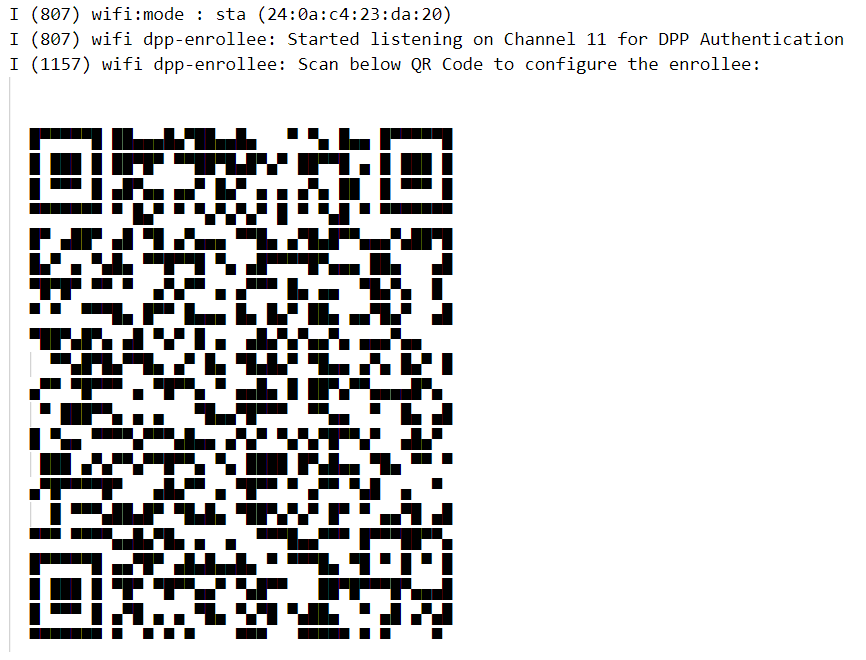
\includegraphics[scale=0.5]{imgs/easy_connect}
	\caption{Primjer QR koda koji generira ESP32 koristeći \textit{Easy Connect}}
	\label{fig:easy_connect}
\end{figure}

ESP-NOW vrsta je bežičnog komunikacijskog protokola tvrtke \textit{Espressif} koji omogućuje izravnu, brzu i niskonaponsku kontrolu pametnih uređaja, bez potrebe za usmjerivačem. Temeljen je na sloju podatkovne veze, koji smanjuje pet slojeva OSI modela na samo jedan. Ovim načinom podaci se ne moraju prenositi kroz ostale slojeve. Također, nema potrebe za zaglavljima paketa ili raspakiranjem na svakom sloju, što dovodi do brzog odgovora smanjujući kašnjenje uzrokovano gubitkom paketa u zagušenim mrežama. Podaci aplikacije enkapsulirani su u okvire različitih dobavljača i zatim se prenose s jednog Wi-Fi uređaja na drugi bez veze.Prednost ovog protokola je manje korištenje resursa i procesorske memorije. Na slici \ref{fig:esp_now} uspoređeni su slojevi modela OSI i ESP-NOW. 

\begin{figure}[ht]
	\centering
	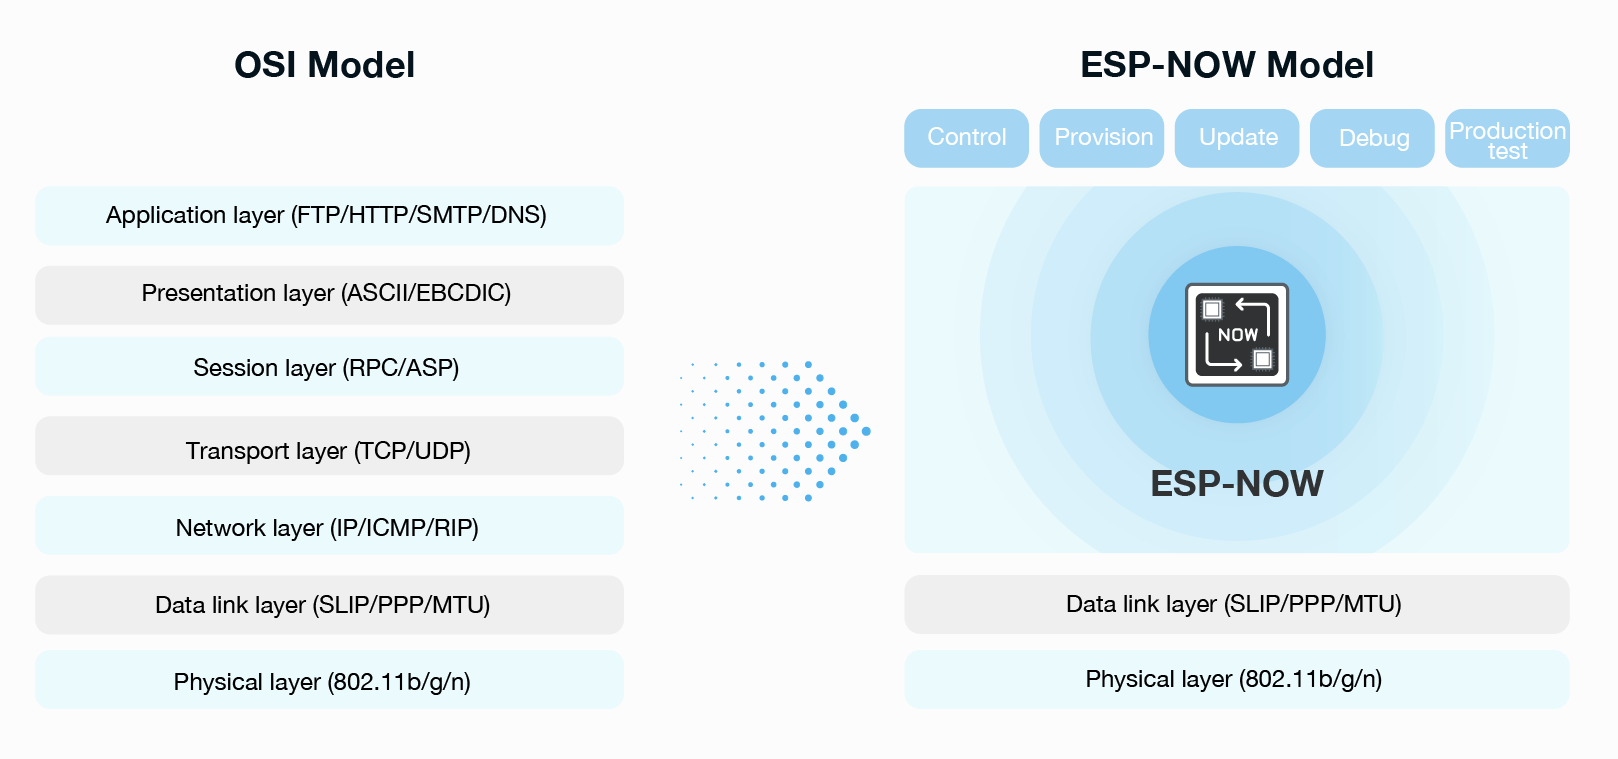
\includegraphics[scale=0.2]{imgs/esp_now}
	\caption{Usporedba modela OSI i ESP-NOW \cite{esp_now}}
	\label{fig:esp_now}
\end{figure}

ESP-TOUCH još je jedan protokol tvrtke \textit{Espressif} koji implementira tehnologiju \textit{Smart Config} za povezivanje modula ESP32 na Wi-Fi mrežu putem jednostavne konfiguracije na pametnog telefonu. Tehnologija \textit{Smart Config} služi za povezivanje novog uređaja u Wi-Fi mrežu. Koristi mobilnu aplikaciju za emitiranje mrežnih vjerodajnica s pametnog telefona na uređaj koji nema pristup Wi-Fi mreži. Prednost ove tehnologije je u tome što uređaj ne mora izravno znati SSID ili lozinku pristupne točke, nego se te informacije dobivaju pomoću pametnog telefona. Ova je tehnologija posebno korisna uređajima bez korisničkog sučelja. Podaci o pristupnoj mreži unose se u aplikaciju koja zatim emitira podatke uređajima u neposrednoj blizini. ESP32 detektira paket, te dohvati konfiguraciju pomoću koje se spoji na Wi-Fi mrežu.

ESP-WIFI-MESH mrežni je protokol i radni okvir za stvaranje bežičnih isprepletenih mreža (engl. \textit{mesh}) pomoću uređaja ESP32 baziran na mrežnoj topologiji veze. Omogućuje modulima da formiraju mrežu u kojoj svaki uređaj djeluje kao čvor i u suradnji s drugim čvorovima proširuje mrežnu pokrivenost te pruža pouzdanu i skalabilnu komunikaciju. ESP-WIFI-MESH razlikuje se od tradicionalnih infrastrukturnih Wi-Fi mreža po tome što se čvorovi ne moraju spajati na središnji čvor. Umjesto toga, čvorovima je dopušteno povezivanje sa susjednim čvorovima. Čvorovi su međusobno odgovorni za međusobni prijenos. To omogućuje mreži puno veće područje pokrivenosti budući da čvorovi još uvijek mogu ostvariti međupovezanost bez potrebe da budu u dometu središnjeg čvora. Isto tako, ova je arhitekturna topologija također manje osjetljiva na preopterećenje budući da broj dopuštenih čvorova na mreži više nije ograničen jednim središnjim čvorom. Čvorovi istovremeno rade kao stanica i pristupna točka, stoga nisu ograničeni klasičnim povezivanjem u jednom ili drugom načinu. Međutim, način rada stanice ograničava modul na spajanje samo sa jednim uređajem, dok se na njega može spojiti više uređaja jer istovremeno radi kao pristupna točka. Ova ograničenja rezultiraju mrežnom strukturom stabla, pri kojem svaki čvor odnosno modul ima jednog roditelja odnosno pristupnu točku na koju je spojen, te nekoliko djece koja su spojena na njega. Na slici \ref{fig:traditional_arch} nalazi se model tradicionalne Wi-Fi arhitekture, dok je na slici \ref{fig:mesh_arch} prikazana \textit{mesh} arhitektura. 

\begin{figure}[ht]
	\begin{minipage}[t]{0.4\textwidth}
		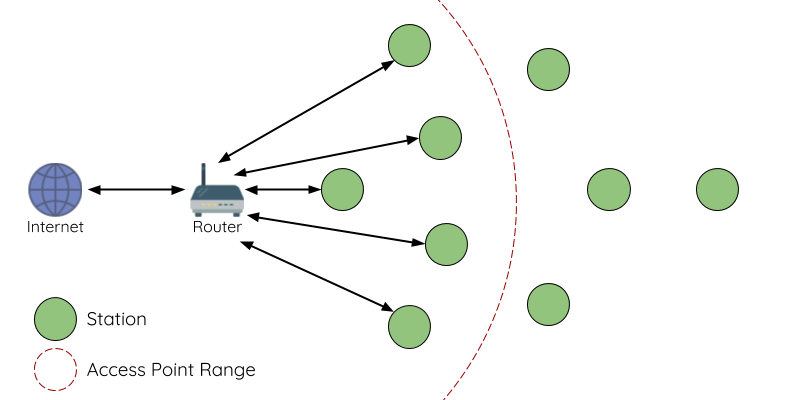
\includegraphics[width=\linewidth]{imgs/traditional_arch}
		\caption{Tradicionalna mrežna arhitektura \cite{espressif}}
		\label{fig:traditional_arch}
	\end{minipage}
	\hspace*{\fill}
	\begin{minipage}[t]{0.4\textwidth}
		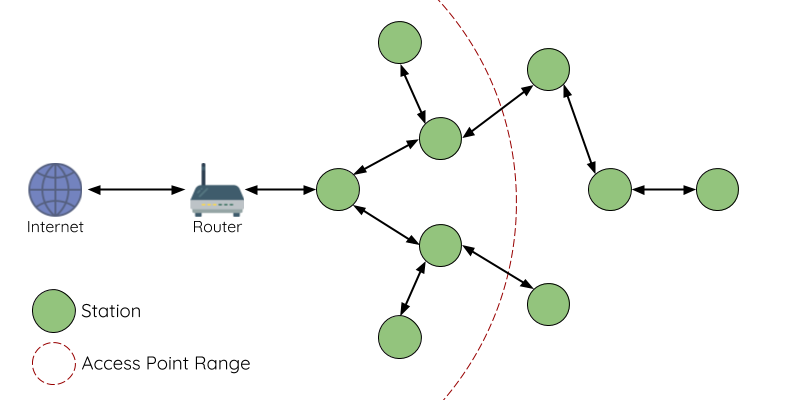
\includegraphics[width=\linewidth]{imgs/mesh_arch}
		\caption{Mrežna arhitektura s \textit{mesh} topologijom \cite{espressif}}
		\label{fig:mesh_arch}
	\end{minipage}
\end{figure}


\section{Sigurnost}

Osim tradicionalnih sigurnosnih metoda poput WEP i WPA2, modul ESP32 nudi podržava i suvremene sigurnosne protokole  kao što su Wi-Fi Protected Access 3 (WPA-Personal) te zaštićeni upravljački okviri (engl. \textit{Protected Management Frames - PMF}). Ove značajke zajedno pružaju bolju privatnost i robusnost protiv poznatih napada na tradicionalne načine rada.

U Wi-Fi mreži, stanice koriste upravljačke okvire kako bi se povezale na pristupnu točku. Za razliku od podatkovnih okvira, ovi se okviri ne šalju kriptirani. Napadač može prisluškivati mrežu i umetnuti lažne pakete kako bi poslao lažne (engl. \textit{spoofed}) okvire u pravom trenutku, što dovodi do sljedećih napada u slučaju nezaštićene razmjene upravljačkih okvira: 

\begin{itemize}
	\item DOS (engl. \textit{Denial of Service}) napad na jednog ili više klijenata,
	\item dohvat SSID-a skrivene mreže,
	\item napad „čovjek u sredini“ (engl. \textit{man-in-the-middle}) pri kojem se klijent odspoji od legitimne pristupne točke i autentificira podatke na lažnoj točki.
\end{itemize}  

PMF pruža zaštitu od ovih napada šifriranjem jednokratnih okvira upravljanja i pružanjem provjere integriteta za emitirane upravljačke okvire. To uključuje deautentifikaciju, odvajanje i robusne upravljačke okvire. Također pruža mehanizam za uklanjanje sigurne asocijacije kako bi se spriječilo da lažni okviri za provjeru autentičnosti prekinu vezu već povezanih klijenata. ESP32-C3 podržava PMF u načinu rada stanice i pristupne točke.

\textit{Wi-Fi Protected Access-3} (WPA3) skup je poboljšanja sigurnosti Wi-Fi pristupa namijenjen za zamjenu trenutnog standarda WPA2. Uključuje nove značajke i mogućnosti koje nude značajno bolju zaštitu od različitih vrsta napada. Trenutno je WPA3 podržan isključivo u načinu rada stanice. WPA3 Poboljšava WPA2-Personal na sljedeće načine:
\begin{itemize}
	\item WPA3 koristi Simultaneous Authentication of Equals (SAE), što je metoda dogovora o ključu s lozinkom koja se temelji na Diffie-Hellman razmjeni ključeva. Za razliku od WPA2, tehnologija je otporna na \textit{offline} napade rječnikom, gdje napadač pokušava odrediti zajedničku lozinku na temelju snimljenog četverosmjernog rukovanja bez ikakve daljnje mrežne interakcije.
	\item Onemogućuje zastarjele protokole koji su osjetljivi na jednostavne napade, primjerice protokol TKIP (engl. \textit{Temporal Key Integrity Protokol}).
	\item Nalaže korištenje PMF-a, čime pruža zaštitu za jednostruke i emitirane upravljačke okvire. To znači da napadač ne može prekinuti uspostavljenu WPA3 sjednicu slanjem krivotvorenih okvira pristupnoj točki ili stanici. 
	\item Pruža unaprijed tajnost, što znači da se snimljeni podaci ne mogu dešifrirati čak i ako je lozinka ugrožena nakon prijenosa podataka. \cite{espressif}
\end{itemize}

\eject